\documentclass[0_main]{subfiles}

\begin{document}

\ifEn
    \subsection{Representative Quasi-Newton Update Rules}
\else
    \subsection{代表的な準ニュートン更新則}
\fi

\ifEn
    Given $B_k$, $s_k$, and $y_k$, there exist many update rules that produce $B_{k+1}$ satisfying the secant condition. We introduce several representative ones together with their derivations~\citep{dennisjr.QuasiNewtonMethodsMotivation1977a}.
    In this subsection only, for brevity, we abbreviate $B_k$, $B_{k+1}$, $s_k$, and $y_k$ as $B$, $\bar{B}$, $s$, and $y$, respectively.
\else
    $B_k$, $s_k$, $y_k$ が与えられたとき、セカント条件を満たす $B_{k+1}$ を与える更新則は多数存在します。ここでは代表的なものをその導出とともに示します~\citep{dennisjr.QuasiNewtonMethodsMotivation1977a}。
    本小節に限り、簡潔さのため $B_k$, $B_{k+1}$, $s_k$, $y_k$ をそれぞれ $B$, $\bar{B}$, $s$, $y$ と略記します。
\fi

\ifEn
    \subsubsection{Broyden's Update}
\else
    \subsubsection{Broyden更新}
\fi

\ifEn
    Broyden's update is one of the oldest known update rules, but it is not often used for quasi-Newton methods in practice due to its lack of symmetry.
    We introduce it briefly for historical context.
    The update formulas are given by
\else
    \href{https://en.wikipedia.org/wiki/Broyden%27s_method}{Broyden更新}は最も古くから知られる更新則の一つですが、準ニュートン法の文脈では、対称性を保たないため実用上はあまり用いられません。歴史的な観点もふまえ、簡潔に紹介します。
    更新則は次で与えられます。
\fi
\begin{equation*}
    \bar{B}_{\mathrm{Broyden}} \coloneqq B + \frac{(y - Bs)s^\top}{s^\top s}.
\end{equation*}

\ifEn
    \paragraph{Derivation}
\else
    \paragraph{導出}
\fi

\ifEn
    We derive this formula from simple structural assumptions~\citep[Section 4]{dennisjr.QuasiNewtonMethodsMotivation1977a}.
\else
    単純な構造的仮定からこの公式を導出します~\citep[Section 4]{dennisjr.QuasiNewtonMethodsMotivation1977a}。
\fi
\begin{proposition}
    \ifEn
        Assume that $\bar{B}$ satisfies the secant condition
        \begin{equation*}
            \bar{B}s = y,
        \end{equation*}
        and the action constraint
        \begin{equation*}
            \bar{B}z = Bz
            \quad\text{for all } z\in\mathbb{R}^n \text{ such that } z^\top s = 0.
        \end{equation*}
        Then $\bar{B}$ is uniquely determined, and it is $\bar{B}_{\mathrm{Broyden}}$.
    \else
        $\bar{B}$ がセカント条件
        \begin{equation*}
            \bar{B}s = y,
        \end{equation*}
        と作用制約
        \begin{equation*}
            \bar{B}z = Bz
            \quad\text{for all } z\in\mathbb{R}^n \text{ such that } z^\top s = 0.
        \end{equation*}
        を満たすと仮定します。このとき $\bar{B}$ は一意に定まり、$\bar{B}_{\mathrm{Broyden}}$ に一致します。
    \fi
\end{proposition}
\begin{proof}
    \ifEn
        A vector $s$ and a basis for the orthogonal complement of $s$ form a basis of $\mathbb{R}^n$.
        Since the conditions on $\bar{B}$ completely determine the action of $\bar{B}$ with respect to this basis, $\bar{B}$ is uniquely determined.

        We now show that $\bar{B}_{\mathrm{Broyden}}$ satisfies the imposed conditions.
        Let $z$ be any vector satisfying $z^\top s = 0$. Then
    \else
        ベクトル $s$ と $s$ の直交補空間の基底は $\mathbb{R}^n$ の基底を成します。
        $\bar{B}$ の条件はこの基底に対する $\bar{B}$ の作用を完全に決定するため、$\bar{B}$ は一意に定まります。

        ここで $\bar{B}_{\mathrm{Broyden}}$ が課された条件を満たすことを示します。
        $z^\top s = 0$ を満たす任意のベクトル $z$ を取ります。このとき、次を得ます。
    \fi
    \begin{align*}
        \bar{B}_{\mathrm{Broyden}} s
         & = \left(B + \frac{(y - Bs)s^\top}{s^\top s}\right) s
        = Bs + (y - Bs)
        = y,                                                    \\
        \bar{B}_{\mathrm{Broyden}} z
         & = \left(B + \frac{(y - Bs)s^\top}{s^\top s}\right) z
        = Bz + (z^\top s) \frac{y - Bs}{s^\top s}
        = Bz.
    \end{align*}
    \ifEn
        Hence $\bar{B}_{\mathrm{Broyden}}$ satisfies the imposed conditions.
        Therefore, by uniqueness, we conclude that $\bar{B} = \bar{B}_{\mathrm{Broyden}}$.
    \else
        したがって、$\bar{B}_{\mathrm{Broyden}}$ は課された条件を満たします。
        よって、一意性より $\bar{B} = \bar{B}_{\mathrm{Broyden}}$ となります。
    \fi
    \myQED
\end{proof}

\ifEn
    Broyden's update can also be characterized as a minimal-change update in the Frobenius norm.
\else
    Broyden更新は、フロベニウスノルムにおける最小変化更新としても特徴づけられます。
\fi

\begin{proposition}[\citep{dennisjr.QuasiNewtonMethodsMotivation1977a}, Theorem~4.1]
    \ifEn
        Let $B\in\mathbb{R}^{n\times n}$, $y\in\mathbb{R}^n$, and $s\in\mathbb{R}^n\setminus\{ 0 \}$ be given.
        Then $\bar{B}_{\mathrm{Broyden}}$ is the unique solution of the following optimization problem:
    \else
        $B\in\mathbb{R}^{n\times n}$, $y\in\mathbb{R}^n$, $s\in\mathbb{R}^n\setminus\{ 0 \}$ が与えられているとき、行列 $\bar{B}_{\mathrm{Broyden}}$ は以下の最適化問題の一意解である。
    \fi
    \begin{align*}
        \underset{\tilde{B} \in \mathbb{R}^{n \times n}}{\mathrm{minimize}} & \quad \lVert \tilde{B} - B \rVert_F \\
        \mathrm{subject to}                                                 & \quad \tilde{B} s = y.
    \end{align*}
\end{proposition}
\begin{proof}
    \ifEn
        Instead of directly solving the optimization problem, we note that we can think of optimizing the function $\tilde{B} \mapsto \lVert \tilde{B} - B \rVert_F^2$, which is convex on $\mathbb{R}^{n \times n}$.
        The constraint set
        \begin{equation*}
            \{\tilde{B}\in\mathbb{R}^{n\times n}:\tilde{B}s=y\}
        \end{equation*}
        is affine and hence convex.
        Therefore, the optimization problem admits at most one minimizer.

        We show that $\bar{B}_{\mathrm{Broyden}}$ is indeed the minimizer.
        For any $\tilde{B}$ satisfying $\tilde{B}s=y$, we have
    \else
        関数 $\tilde{B}\mapsto\lVert \tilde{B}-B \rVert^2_F$ を最適化すると考えてよく、これは $\mathbb{R}^{n\times n}$ 上で凸です。
        制約集合
        \begin{equation*}
            \{\tilde{B}\in\mathbb{R}^{n\times n}:\tilde{B}s=y\}
        \end{equation*}
        はアフィン集合であり凸です。
        よって、この最適化問題は高々一つの最小解しか持ちません。

        $\bar{B}_{\mathrm{Broyden}}$ が実際に最小解であることを示します。
        制約 $\tilde{B}s=y$ を満たす任意の $\tilde{B}$ に対して
    \fi
    \begin{equation*}
        \lVert \bar{B}_{\mathrm{Broyden}} - B \rVert_F^2
        = \left\lVert (\tilde{B}-B) \frac{s s^\top}{s^\top s} \right\rVert_F^2
        \leq \lVert \tilde{B}-B \rVert_F^2.
    \end{equation*}
    \ifEn
        We used the submultiplicativity of the Frobenius norm and the fact that $\lVert ss^\top/(s^\top s) \rVert_F=1$.
        Hence $\tilde{B}=\bar{B}_{\mathrm{Broyden}}$.
    \else
        ここでフロベニウスノルムの劣乗法性と $\lVert ss^\top/(s^\top s) \rVert_F=1$ を用いました。
        よって $\tilde{B}=\bar{B}_{\mathrm{Broyden}}$ です。
    \fi
    \myQED
\end{proof}

\ifEn
    Note that this update rule does not preserve symmetry. In the following, we introduce representative quasi-Newton update rules that improve upon this aspect.
\else
    この更新則は、対称性を保たないという点に注意してください。以下では、その点を改善した代表的な準ニュートン更新則を紹介します。
\fi

\ifEn
    \subsubsection{Symmetric Rank-One (SR1) Update}
\else
    \subsubsection{Symmetric Rank-One (SR1) 更新}
\fi

\ifEn
    The Symmetric Rank-One (SR1) update~\citep{nocedal1999numerical} is a fundamental quasi-Newton method that maintains symmetry throughout the update process. The update formulas are given by
\else
    \href{https://en.wikipedia.org/wiki/Symmetric_rank-one}{対称ランク1 (SR1) 更新}~\citep{nocedal1999numerical} は更新過程で対称性を維持する基本的な準ニュートン法です。更新則は次で与えられます。
\fi
\begin{equation*}
    \bar{B}_{\mathrm{SR1}} \coloneqq B + \frac{(y - B s)(y - B s)^\top}{(y - B s)^\top s}.
\end{equation*}

\ifEn
    \paragraph{Derivation}
\else
    \paragraph{導出}
\fi

\ifEn
    To derive SR1 update, we construct the updated matrix $\bar{B}$ as a rank-one update.
    That is, we assume that for some vector $z \in \mathbb{R}^n$,
\else
    SR1 更新を導出するため、更新行列 $\bar{B}$ をランク1更新として構成します。すなわち、あるベクトル $z \in \mathbb{R}^n$ に対して、次が満たされると仮定します。
\fi
\begin{equation*}
    \bar{B}_{\mathrm{SR1}} = B + z z^\top.
\end{equation*}
\ifEn
    To satisfy the secant condition $\bar{B}_{\mathrm{SR1}} s = y$, when $z^\top s \neq 0$, we need
\else
    セカント条件 $\bar{B}_{\mathrm{SR1}} s = y$ を満たすためには、$z^\top s \neq 0$ のとき、次が必要となります。
\fi
\begin{equation*}
    B s + z z^\top s = y.
\end{equation*}
\ifEn
    Rearranging this equation gives
\else
    整理すると、
\fi
\begin{equation*}
    z = \frac{y - B s}{z^\top s}.
\end{equation*}
\ifEn
    To determine $z^\top s$, we take the inner product with $s$:
\else
    $z^\top s$ を決めるために $s$ との内積を取ると、
\fi
\begin{equation*}
    z^\top s = \frac{(y - B s)^\top s}{z^\top s}.
\end{equation*}
\ifEn
    Rearranging this equation yields the key relation
\else
    この式を整理すると次の関係が得られます。
\fi
\begin{equation*}
    (z^\top s)^2 = (y - B s)^\top s.
\end{equation*}
\ifEn
    Thus, we obtain
\else
    従って、
\fi
\begin{equation*}
    \bar{B}_{\mathrm{SR1}}
    = B + z z^\top
    = B + \frac{(y - B s)(y - B s)^\top}{(z^\top s)^2}
    = B + \frac{(y - B s)(y - B s)^\top}{(y - B s)^\top s}.
\end{equation*}
\ifEn
    Thus, we have derived the SR1 update formula.
    We omit the derivation of $\bar{H}_{\mathrm{SR1}}$.
\else
    よって、SR1 更新則が導出されました。
\fi

\ifEn
    \paragraph{Remarks}
\else
    \paragraph{補足}
\fi

\ifEn
    The SR1 update requires $(y - Bs)^\top s \neq 0$ to be well-defined. When $(y - Bs)^\top s = 0$, the denominator of the SR1 update vanishes, and the update is typically skipped in practice.
\else
    SR1 更新は $(y - Bs)^\top s \neq 0$ であることを前提としています。$(y - Bs)^\top s = 0$ のとき分母が零となり、実用上は更新をスキップすることが多いです。
\fi

\ifEn
    \subsubsection{Powell Symmetric Broyden (PSB) Update}
\else
    \subsubsection{Powell Symmetric Broyden (PSB) 更新}
\fi

\ifEn
    The Powell Symmetric Broyden (PSB) update~\cite{m.j.d.powellNewAlgorithmUnconstrained1970,doi:10.1137/1.9781611971200,haeltermanAnalyticalStudyLeast2009} is also a quasi-Newton update rule. The update formulas are given by
\else
    Powell Symmetric Broyden (PSB) 更新~\cite{m.j.d.powellNewAlgorithmUnconstrained1970,doi:10.1137/1.9781611971200,haeltermanAnalyticalStudyLeast2009} も準ニュートン更新則の一つで、更新則は次で与えられます。
\fi
\begin{equation*}
    \bar{B}_{\mathrm{PSB}} = B + \frac{(y - B s) s^\top + s (y - B s)^\top}{s^\top s} - \frac{s^\top (y - B s)}{(s^\top s)^2} s s^\top
\end{equation*}

\ifEn
    \paragraph{Derivation}
\else
    \paragraph{導出}
\fi

\ifEn
    Recall that the SR1 update adds an update term as $z z^\top$.
    Instead, we can consider an asymmetric rank-one update of the form $z c^\top$ for some vector $c \in \mathbb{R}^n$. We symmetrize the result at the end.
\else
    SR1 更新では更新項を $z z^\top$ として加えていました。代わりに、あるベクトル $c \in \mathbb{R}^n$ に対して、非対称なランク1更新 $z c^\top$ を考えることができます。そして最後に結果を対称化します。
\fi
\ifEn
    Assume $c^\top s \neq 0$, and from $Bs + z c^\top s = y$, we can derive $z$ as
\else
    $c^\top s \neq 0$ と仮定し、$Bs + z c^\top s = y$ から $z$ を
\fi
\begin{equation*}
    z = \frac{y - B s}{c^\top s}
\end{equation*}
\ifEn
    and perform the asymmetric update
\else
    と導き、これを用いて次の非対称更新を行います。
\fi
\begin{equation*}
    C_1 \coloneqq B + \frac{(y - B s)c^\top}{c^\top s}.
\end{equation*}
\ifEn
    Since $C_1$ is generally not symmetric, we symmetrize it via
\else
    $C_1$ は一般に対称でないため、これを対称化します。
\fi
\begin{equation*}
    C_2 = \frac{C_1 + C_1^\top}{2}.
\end{equation*}
\ifEn
    However, the symmetrized matrix $C_2$ may not satisfy the secant condition $C_2 s = y$. Therefore, we iterate this process:
\else
    しかし、対称化された行列 $C_2$ はセカント条件 $C_2 s = y$ を満たさない場合があります。そこでこの過程を反復することを考えます。
\fi
\begin{equation*}
    \begin{dcases}
        C_0 = B                                                                               \\
        C_{2t+1} = C_{2t} + \frac{(y - C_{2t}s)c^\top}{c^\top s} & (\text{asymmetric update}) \\
        C_{2t+2} = \frac{C_{2t+1} + C_{2t+1}^\top}{2}            & (\text{symmetrization})
    \end{dcases}
\end{equation*}
\ifEn
    The key result is that the sequence $\{ C_{2t} \}_{t=0}^{\infty}$ converges to a symmetric matrix satisfying the secant condition, as formalized in the following proposition.
\else
    重要な結果として、列 $\{ C_{2t} \}_{t=0}^{\infty}$ はセカント条件を満たす対称行列に収束します。次の命題ではそれを示します。
\fi

\begin{proposition}[\citep{dennisjr.QuasiNewtonMethodsMotivation1977a}, Lemma~7.2]\label{prop:psb-convergence}
    \ifEn
        The sequence $\{ C_{t} \}_{t=0}^{\infty}$ converges, and the limit is given by
    \else
        行列の列 $\{ C_{t} \}_{t=0}^{\infty}$ は収束し、その極限は次で与えられる。
    \fi
    \begin{equation*}
        \lim_{t \to \infty} C_{t}
        =
        C_{\infty}
        \coloneqq
        B + \frac{(y - Bs)c^\top + c(y - Bs)^\top}{c^\top s} - \frac{(y - Bs)^\top s}{(c^\top s)^2} c c^\top.
    \end{equation*}
\end{proposition}
\begin{proof}
    \ifEn
        We first analyze the even subsequence.
        For $t=0,1,2,\dots$, we define
    \else
        まず偶数番目の部分列を解析します。 $t=0,1,2,\dots$ に対し、次のように定義します。
    \fi
    \begin{equation*}
        G_t \coloneqq C_{2t}.
    \end{equation*}
    \ifEn
        By construction, each $G_t$ is symmetric.
        From the definitions, we have
    \else
        構成方法より各 $G_t$ は対称です。
        定義から次を得ます。
    \fi
    \begin{equation*}
        G_{t+1} = G_t +\frac{1}{2c^\top s}\left((y-G_t s)c^\top+c(y-G_t s)^\top\right).
    \end{equation*}
    \ifEn
        Let us introduce the error vector for the secant condition:
    \else
        また、セカント条件に対する誤差ベクトルを次で導入します。
    \fi
    \begin{equation*}
        w_t \coloneqq y-G_t s.
    \end{equation*}
    \ifEn
        Then, we have
    \else
        このとき、
    \fi
    \begin{equation*}
        G_{t+1} = G_t+\frac{1}{2c^\top s}(w_t c^\top+cw_t^\top).
    \end{equation*}
    \ifEn
        Substituting the above equation into the definition of $w_t$ yields
    \else
        上式を $w_t$ の定義に代入すると
    \fi
    \begin{align*}
        w_{t+1} & = y-\left(G_t+\frac{1}{2c^\top s}(w_t c^\top+cw_t^\top)\right)s \\
                & =
        w_t-\frac12w_t-\frac{w_t^\top s}{2c^\top s}c                              \\
                & =
        \frac{1}{2}\left(w_t-\frac{w_t^\top s}{c^\top s}c\right).
    \end{align*}
    \ifEn
        Hence, we have
    \else
        よって
    \fi
    \begin{equation*}
        w_{t+1}=Pw_t,
        \qquad
        P \coloneqq \frac{1}{2}\left(I-\frac{cs^\top}{c^\top s}\right).
    \end{equation*}
    \ifEn
        The matrix $cs^\top/c^\top s$ is rank one and has eigenvalues $1,0,\dots,0$.
        Therefore, $P$ has one eigenvalue $0$ and all remaining eigenvalues equal to $1/2$.
        In particular, its spectral radius is $1/2<1$, and thus the series converges as follows:
    \else
        行列 $cs^\top/c^\top s$ はランク1で固有値は $1,0,\dots,0$ です。
        よって $P$ は固有値 $0$ を一つ持ち、残りはすべて $1/2$ となります。
        特にスペクトル半径は $1/2<1$ であるので、次のように級数が収束します。
    \fi
    \begin{align*}
        \sum_{t=0}^{\infty}w_t & =        \sum_{t=0}^{\infty}P^t(y-Bs)                         &  & (w_0=y-Bs)                \\
                               & =  (I-P)^{-1}(y-Bs)                                                                          \\
                               & = 2\left(I-\frac{1}{2}\frac{cs^\top}{c^\top s}\right) (y-Bs). &  & (\text{definition of } P)
    \end{align*}
    \ifEn
        Note that the last equation follows from
    \else
        最後の式は次から導かれることに注意してください。
    \fi
    \begin{equation*}
        2(I-P) \left(I-\frac{1}{2}\frac{cs^\top}{c^\top s}\right) = \left(I + \frac{cs^\top}{c^\top s}\right) \left(I-\frac{1}{2}\frac{cs^\top}{c^\top s}\right) = I.
    \end{equation*}
    \ifEn
        Hence, we have
    \else
        よって
    \fi
    \begin{align*}
        \lim_{t\to\infty}G_t
         & =
        B+\frac{1}{2c^\top s}
        \sum_{t=0}^{\infty}(w_t c^\top+c w_t^\top)                                                                                                                                        \\
         & = B+ \left(\sum_{t=0}^{\infty}w_t\right) \frac{c^\top}{2c^\top s} + \frac{c}{2c^\top s} \left(\sum_{t=0}^{\infty}w_t\right)^\top                                               \\
         & = B+ 2\left(I-\frac{1}{2}\frac{cs^\top}{c^\top s}\right) (y-Bs) \frac{c^\top}{2c^\top s} + \frac{c}{2c^\top s} 2(y-Bs)^\top \left(I-\frac{1}{2}\frac{sc^\top}{c^\top s}\right) \\
         & = B + \frac{(y - Bs)c^\top + c(y - Bs)^\top}{c^\top s} - \frac{(y - Bs)^\top s}{(c^\top s)^2} c c^\top                                                                         \\
         & = C_{\infty}.
    \end{align*}
    \ifEn
        This shows the convergence of the even subsequence $\{ C_{2t} \}$ to $C_{\infty}$.

        Next, for the odd subsequence, we have
    \else
        これで偶数番目の部分列 $\{ C_{2t} \}$ が $C_{\infty}$ に収束することが示されました。

        次に奇数番目の部分列について、次の式が成立しています。
    \fi
    \begin{equation*}
        C_{2t+1}
        =
        G_t+\frac{w_t c^\top}{c^\top s}.
    \end{equation*}
    \ifEn
        Since $G_t\to C_{\infty}$ and $\lVert w_t \rVert\to0$ from the spectral radius of $P$ being less than one, we have
    \else
        $G_t\to C_{\infty}$ であり、また $\lVert w_t \rVert\to0$ が $P$ のスペクトル半径が1未満であることから従うため、
    \fi
    \begin{equation*}
        C_{2t+1} \to C_{\infty}.
    \end{equation*}
    \ifEn
        Therefore both subsequences $\{ C_{2t} \}$ and $\{ C_{2t+1} \}$ converge to $C_{\infty}$, completing the proof.
    \else
        従って、部分列 $\{ C_{2t} \}$ と $\{ C_{2t+1} \}$ はどちらも $C_{\infty}$ に収束し、証明が完了します。
    \fi
    \myQED
\end{proof}

\ifEn
    When $c = s$, the general formula of $C_{\infty}$ simplifies to the standard PSB update formula:
\else
    $c = s$ のとき、$C_{\infty}$ の一般式は標準的な PSB 更新則を導きます。
\fi
\begin{equation*}
    \bar{B}_{\mathrm{PSB}} = B + \frac{(y - Bs)s^\top + s(y - Bs)^\top}{s^\top s} - \frac{(y - Bs)^\top s}{(s^\top s)^2} ss^\top.
\end{equation*}

\ifEn
    \subsubsection{Davidon--Fletcher--Powell (DFP) Update}
\else
    \subsubsection{Davidon--Fletcher--Powell (DFP) 更新}
\fi

\ifEn
    The Davidon--Fletcher--Powell (DFP) update~\cite{nocedal1999numerical} is also a classical quasi-Newton update formula. The update formulas are given by
\else
    \href{https://en.wikipedia.org/wiki/Davidon%E2%80%93Fletcher%E2%80%93Powell_formula}{Davidon--Fletcher--Powell (DFP) 更新}~\cite{nocedal1999numerical} も古典的な準ニュートン更新則です。
    更新則は次で与えられます。
\fi
\begin{equation*}
    \bar{B}_{\mathrm{DFP}} = \left(I - \frac{y s^\top}{y^\top s}\right) B \left(I - \frac{s y^\top}{y^\top s}\right) + \frac{y y^\top}{y^\top s}.
\end{equation*}

\ifEn
    \paragraph{Derivation}
\else
    \paragraph{導出}
\fi

\ifEn
    In the PSB update rule discussed earlier, we substituted $c=s$, but we can consider taking a different $c$. Specifically, substituting $c=y$ yields the DFP update as follows.
\else
    先に述べた PSB 更新では $c=s$ としましたが、別の $c$ を選ぶことも可能です。
    具体的には $c=y$ を代入すると次のように DFP 更新が得られます。
\fi
\begin{equation*}
    \bar{B}_{\mathrm{DFP}} = B + \frac{(y - Bs)y^\top + y(y - Bs)^\top}{y^\top s} - \frac{(y - Bs)^\top s}{(y^\top s)^2} yy^\top.
\end{equation*}
\ifEn
    There are other derivations of the DFP update, some of which can be understood as dual versions of the derivation of the subsequent BFGS update.
\else
    なお、DFP更新には他にも導出方法が存在し、それらの一部は、次のBFGS更新における導出の双対版として理解することもできます。
\fi

\ifEn
    \subsubsection{Broyden--Fletcher--Goldfarb--Shanno (BFGS) Update}
\else
    \subsubsection{Broyden--Fletcher--Goldfarb--Shanno (BFGS) 更新}
\fi

\ifEn
    The Broyden--Fletcher--Goldfarb--Shanno (BFGS) update is one of the most widely used quasi-Newton methods. The update formulas are given by
\else
    \href{https://en.wikipedia.org/wiki/Broyden%E2%80%93Fletcher%E2%80%93Goldfarb%E2%80%93Shanno_algorithm}{Broyden--Fletcher--Goldfarb--Shanno (BFGS) 更新}は最も広く使われる準ニュートン法の一つです。
    更新則は次で与えられます。
\fi
\begin{equation*}
    \bar{B}_{\mathrm{BFGS}} = B - \frac{B s s^\top B}{s^\top B s} + \frac{y y^\top}{y^\top s}
\end{equation*}

\ifEn
    \paragraph{Derivation by Duality}
\else
    \paragraph{双対による導出}
\fi

\ifEn
    This update can be derived by considering the dual of the DFP update.
    As we will see later, the BFGS update with respect to $B$ has the same form as the DFP update with respect to $H$.
\else
    この更新はDFP更新の双対を考えることで導出できます。
    後で示すように、$B$ に対するBFGS更新は $H$ に対する DFP 更新と同じ形式となっています。
\fi

\ifEn
    \paragraph{Derivation by KL Divergence Minimization}
\else
    \paragraph{KLダイバージェンス最小化による導出}
\fi

\ifEn
    The KL divergence is a non-symmetric measure of proximity between matrices.
    For positive definite matrices $P,Q \in \mathbb{R}^{n \times n}$, it is defined by
\else
    KLダイバージェンスとは、行列間の近さを測る一種の非対称な尺度です。
    正定値行列 $P,Q \in \mathbb{R}^{n \times n}$ に対して、次で定義されます。
\fi
\begin{equation*}
    \mathrm{KL}(P,Q) \coloneqq \mathrm{tr}(P Q^{-1}) - \log\det(P Q^{-1}) - n.
\end{equation*}
\ifEn
    Let $T \in \mathbb{R}^{n \times n}$ be an arbitrary nonsingular matrix.
    Since the trace is invariant under cyclic permutations, the KL divergence satisfies
\else
    行列 $T \in \mathbb{R}^{n \times n}$ を任意の正則行列とします。
    $\mathrm{tr}$ は2つの行列の積に対して可換性を持つため、KLダイバージェンスは次の不変性を持ちます。
\fi
\begin{align*}
    \mathrm{KL}(T P T^\top, T Q T^\top) & = \mathrm{tr}(T P T^\top (T Q T^\top)^{-1}) - \log\det(T P T^\top (T Q T^\top)^{-1}) - n \\
                                        & = \mathrm{tr}(P Q^{-1} T^{-1} T) - \log (\det(T) \det(P Q^{-1}) \det(T^{-1})) - n        \\
                                        & = \mathrm{tr}(P Q^{-1}) - \log\det(P Q^{-1}) - n                                         \\
                                        & = \mathrm{KL}(P, Q).
\end{align*}

\ifEn
    It is known that the BFGS update can be obtained as the solution to the following KL divergence minimization problem:
\else
    ここで、BFGS更新は次のKLダイバージェンス最小化問題の解として得られることが知られています。
\fi
\begin{align*}
    \underset{\bar{B} \succ 0}{\mathrm{minimize}}
     & \quad \mathrm{KL}(\bar{B}, B) \\
    \mathrm{subject\ to}
     & \quad \bar{B}s = y.
\end{align*}

\begin{proposition}[{\citep[Section 7.2.4]{kanamori2016continuous}}]
    \ifEn
        Let $B \succ 0$ be a symmetric positive definite matrix.
        The solution to the above optimization problem is given by the BFGS update formula.
    \else
        $B \succ 0$ を正定値対称行列とする。
        このとき、上記の最適化問題の解はBFGS更新則で与えられる。
    \fi
\end{proposition}
\begin{proof}
    \ifEn
        Since $B$ is a symmetric positive definite matrix, we first define
    \else
        $B$ が正定値対称行列であることに注意して、
        まず、次のように定義します。
    \fi
    \begin{equation*}
        s' \coloneqq B^{\frac{1}{2}} s, \quad y' \coloneqq B^{-\frac{1}{2}} y, \quad B' \coloneqq B^{-\frac{1}{2}} \bar{B} B^{-\frac{1}{2}}.
    \end{equation*}
    \ifEn
        Then, the optimization problem can be rewritten as
    \else
        すると、最適化問題は次のように書き直せます。
    \fi
    \begin{align*}
        \underset{B' \succ 0}{\text{minimize}} & \quad \mathrm{KL}(B', I) \\
        \text{subject to}                      & \quad B' s' = y'.
    \end{align*}
    \ifEn
        Here, we used the invariance of the KL divergence:
    \else
        ただし、KLダイバージェンスの不変性より、次が成り立つことを用いました。
    \fi
    \begin{equation*}
        \mathrm{KL}(\bar{B}, B) = \mathrm{KL}(B^{-\frac{1}{2}} \bar{B} B^{-\frac{1}{2}}, B^{-\frac{1}{2}} B B^{-\frac{1}{2}}) = \mathrm{KL}(B', I)
    \end{equation*}
    \ifEn
        Note that the constraint $B' \succ 0$ automatically includes symmetry, so adding the constraint $B' = B'^\top$ explicitly does not change the solution.
    \else
        なお、本最適化問題において $B' \succ 0$ という制約は自動的に対称性を含むため、$B' = B'^\top$ を制約として陽に課しても解は変わりません。
    \fi


    \ifEn
        Let us solve this problem using the method of Lagrange multipliers.
        We introduce the Lagrange multipliers $\lambda \in \mathbb{R}^n$ and $\Lambda \in \mathbb{R}^{n \times n}$, and define the Lagrangian as
    \else
        この問題の解を、ラグランジュの未定乗数法を用いて求めます。
        ラグランジュ乗数 $\lambda\in\mathbb{R}^n$ および $\Lambda\in\mathbb{R}^{n\times n}$ を用いて、ラグランジアンを次のように定義します。
    \fi
    \begin{equation*}
        \mathcal{L}(B',\lambda,\Lambda) = \mathrm{tr}(B') -\log\det(B') -n +2\lambda^\top(B's'-y') +\mathrm{tr}\left(\Lambda(B'-B'^\top)\right).
    \end{equation*}
    \ifEn
        In general, for matrix differentiation, the derivative of $\log\det(X)$ with respect to $X$ for $X \succ 0$ is $X^{-\top}$, and the derivative of $\mathrm{tr}(AX)$ is $A^\top$.
        By differentiating with respect to $B'$ and using $B' = B'^\top$, we can write down the stationarity condition of the KKT conditions as follows:
    \else
        一般に、行列微分の公式として、$X \succ 0$ に対して、$\log\det(X)$ の微分が $X^{-\top}$ かつ、 $\mathrm{tr}(AX)$ の微分が $A^\top$ となります。
        KKT条件のうち停留性に関する条件は、$B'$ で微分し、$B'=B'^\top$ を用いることで次のように書けます。
    \fi
    \begin{equation*}
        I-B'^{-\top}
        +2\lambda s'^\top
        +\Lambda^\top-\Lambda
        =0.
    \end{equation*}
    \ifEn
        By adding this equation and its transpose, and dividing by 2 again using $B' = B'^\top$, we obtain
    \else
        この式とその転置を加えて2で割り、再び $B' = B'^\top$ を用いると次を得る。
    \fi
    \begin{equation*}
        B'^{-1} = I+\lambda s'^\top+s'\lambda^\top.
    \end{equation*}
    \ifEn
        By the constraint $B's' = y'$, we have $B'^{-1}y' = s'$, so multiplying the above equation by $y'$ from the right and then by $y'^\top$ from the left yields
    \else
        制約条件 $B's'=y'$ より $B'^{-1}y'=s'$ であるから、
        上式に右から $y'$ を掛けた式と、さらに左から $y'^\top$ を掛けた式はそれぞれ、次のようになる。
    \fi
    \begin{align*}
        s'         & = y' +(s'^\top y')\lambda +(\lambda^\top y')s'                                \\
        y'^\top s' & = y'^\top y' + (s'^\top y')(y'^\top \lambda) + (\lambda^\top y')(y'^\top s').
    \end{align*}
    \ifEn
        From the second equation, we have
    \else
        第2式より
    \fi
    \begin{equation*}
        \lambda^\top y'
        =
        \frac{y'^\top s'-y'^\top y'}{2(s'^\top y')}.
    \end{equation*}
    \ifEn
        Substituting this into the first equation gives
    \else
        これを第1式に代入すると、
    \fi
    \begin{equation*}
        \lambda
        = \frac{s'-y'}{s'^\top y'} - \frac{\lambda^\top y'}{s'^\top y'}s'
        =
        \frac{s'^\top y'+y'^\top y'}{2(s'^\top y')^2}s'
        -\frac{1}{s'^\top y'}y'.
    \end{equation*}
    \ifEn
        By substituting this $\lambda$ into the expression for $B'^{-1}$ and simplifying, we obtain
    \else
        この $\lambda$ を $B'^{-1}$ の表式に代入して整理すると、
    \fi
    \begin{align*}
        B'^{-1} & = I + 2\frac{s'^\top y'+y'^\top y'}{2(s'^\top y')^2}(s' s'^\top)
        -\frac{1}{s'^\top y'}(y' s'^\top + s' y'^\top)                                                                                         \\
                & = \left( I-\frac{s'y'^\top}{s'^\top y'} \right) \left( I-\frac{y's'^\top}{s'^\top y'} \right) +\frac{s's'^\top}{s'^\top y'}.
    \end{align*}
    \ifEn
        Finally, since $B' = B^{-\frac{1}{2}} \bar{B} B^{-\frac{1}{2}}$, we have $\bar{B} = B^{\frac{1}{2}} B' B^{\frac{1}{2}}$, and thus calculating $\bar{B}^{-1}$ gives
    \else
        最後に $B' = B^{-\frac{1}{2}} \bar{B} B^{-\frac{1}{2}}$ より、$\bar{B} = B^{\frac{1}{2}} B' B^{\frac{1}{2}}$ であるため、$\bar{B}^{-1}$ を計算すると、
    \fi
    \begin{align*}
        \bar{B}^{-1} & = B^{-\frac{1}{2}} B'^{-1} B^{-\frac{1}{2}}                                                                                                                                                                          \\
                     & = B^{-\frac{1}{2}} \left( I-\frac{s'y'^\top}{s'^\top y'} \right) \left( I-\frac{y's'^\top}{s'^\top y'} \right) B^{-\frac{1}{2}} + \frac{(B^{-\frac{1}{2}}s')(B^{-\frac{1}{2}}s')^\top}{s'^\top y'}                   \\
                     & = B^{-\frac{1}{2}} \left( I-\frac{B^{\frac{1}{2}}s y^\top B^{-\frac{1}{2}}}{s^\top y} \right) \left( I-\frac{B^{-\frac{1}{2}}y s^\top B^{\frac{1}{2}}}{s^\top y} \right) B^{-\frac{1}{2}} + \frac{ss^\top}{s^\top y} \\
                     & = \left( I - \frac{s y^\top}{y^\top s} \right) B^{-1} \left( I - \frac{y s^\top}{y^\top s} \right) + \frac{s s^\top}{y^\top s}.
    \end{align*}
    \ifEn
        As we will see later, this is indeed the formula for the inverse of the BFGS update, which completes the proof.
    \else
        後述の通り、これは確かにBFGS更新の逆行列の公式であるため、証明が完了します。
    \fi
    \myQED
\end{proof}

\ifEn
    As for more details, see \citep{kanamoriBregmanExtensionQuasiNewton2010,kanamoriBregmanExtensionQuasiNewton2010a}.
\else
    更なる詳細については
    \citep{kanamoriBregmanExtensionQuasiNewton2010,kanamoriBregmanExtensionQuasiNewton2010a}
    をご参照ください。
    \href{http://matsuzoe.web.nitech.ac.jp/infogeo/OCAMI2010/kanamori.pdf}{こちらのスライド}
    も参考になります。
\fi


\ifEn
    \subsection{Details of BFGS Update}
\else
    \subsection{BFGS更新の詳細}
\fi

\ifEn
    In this subsection, we focus on the BFGS update and provide a detailed derivation of its formula.
    BFGS update is known as one of the most successful quasi-Newton update rules in practice.
    Recall that the BFGS update formula is given by
\else
    本小節ではBFGS更新に注目し、その公式の詳細な導出を示します。
    BFGS更新は実用上最も成功した準ニュートン更新則の一つとして知られています。
    BFGS更新則は次で与えられていたことを再掲しておきます。
\fi
\begin{equation*}
    B_{k+1}   = B_k - \frac{B_k s_k s_k^\top B_k}{s_k^\top B_k s_k} + \frac{y_k y_k^\top}{y_k^\top s_k}.
\end{equation*}

\ifEn
    \subsubsection{Formula for the Inverse Update}
\else
    \subsubsection{逆更新の公式}
\fi

\ifEn
    The inverse of the BFGS update $H_k \coloneqq B_k^{-1}$ is given by
\else
    BFGS更新の逆行列 $H_k \coloneqq B_k^{-1}$ は次式で与えられます。
\fi
\begin{equation*}
    H_{k+1} = \left(I - \frac{s_k y_k^\top}{y_k^\top s_k}\right) H_k \left(I - \frac{y_k s_k^\top}{y_k^\top s_k}\right) + \frac{s_k s_k^\top}{y_k^\top s_k}.
\end{equation*}
\ifEn
    Note that this BFGS update formula for $H_{k+1}$ has the same form as the DFP update formula for $B_{k+1}$. These are dual to each other.
    We now prove that this equation indeed gives the inverse of the BFGS update.
\else
    なお、このBFGS更新における $H_{k+1}$ の公式は、DFP更新則における $B_{k+1}$ の形式と同じであることに注意してください。これらは双対の関係にあります。
    以下では、この式が確かにBFGS更新の逆行列を与えることを示します。
\fi

\begin{proposition}
    \ifEn
        The matrix $H_{k+1}$ is the inverse of $B_{k+1}$.
    \else
        行列 $H_{k+1}$ は $B_{k+1}$ の逆行列である。
    \fi
\end{proposition}
\begin{proof}
    \ifEn
        The BFGS update can be rewritten in a compact rank-two form
    \else
        BFGS更新は次の簡潔なランク2の形に書き直せます。
    \fi
    \begin{equation*}
        B_{k+1} = B_k + UCV^\top.
    \end{equation*}
    \ifEn
        Here, we define
    \else
        ここで
    \fi
    \begin{equation*}
        U = \begin{bmatrix}B_k s_k & y_k\end{bmatrix},\qquad
        C = \begin{pmatrix}-\frac{1}{s_k^\top B_k s_k} & 0 \\ 0 & \frac{1}{y_k^\top s_k}\end{pmatrix},\qquad
        V = \begin{bmatrix}B_k s_k & y_k\end{bmatrix}
    \end{equation*}
    \ifEn
        since
    \else
        です。実際、次の式が成り立ちます。
    \fi
    \begin{equation*}
        U C V^\top   = \begin{bmatrix} -\frac{B_k s_k}{s_k^\top B_k s_k}&    \frac{y_k}{y_k^\top s_k} \end{bmatrix} \begin{bmatrix} s_k^\top B_k  \\  y_k^\top \end{bmatrix}
        = -\frac{B_k s_k s_k^\top B_k}{s_k^\top B_k s_k} + \frac{y_k y_k^\top}{y_k^\top s_k}.
    \end{equation*}
    \ifEn
        By the Sherman--Morrison--Woodbury identity, we can compute $H_{k+1}$ as follows:
    \else
        Sherman--Morrison--Woodbury の恒等式より、$H_{k+1}$ を次のように計算できます。
    \fi
    \begin{align*}
        H_{k+1} & = (B_k + U C V^\top)^{-1}                                                                                                                                                                                                                                                                                                                                                                                                                                                                                                                                                                                                                                                                      \\
                & = B_k^{-1}- B_k^{-1}U\left(C^{-1}+V^\top B_k^{-1}U\right)^{-1}V^\top B_k^{-1}                                                                                                                                                                                                                                                                                                                                                                                                                                                                                                                                                                                                                  \\
                & = H_k- \begin{bmatrix}s_k & H_k y_k\end{bmatrix} \left(\begin{pmatrix}- s_k^\top B_k s_k & 0                                                                                                                                                                                                                                            \\0    & y_k^\top s_k\end{pmatrix}+\begin{pmatrix}s_k^\top B_k s_k   & s_k^\top y_k      \\y_k^\top s_k & y_k^\top H_k y_k\end{pmatrix}\right)^{-1}\begin{bmatrix}s_k^\top \\ y_k^\top H_k\end{bmatrix}                                                                                                                                                \\
                & = H_k- \begin{bmatrix}s_k                                                                                                                             & H_k y_k\end{bmatrix}\begin{pmatrix}0                                                               & y_k^\top s_k                                                                                                                                                                                                                                          \\y_k^\top s_k       & y_k^\top H_k y_k + y_k^\top s_k\end{pmatrix}^{-1}\begin{bmatrix}s_k^\top                         \\     y_k^\top H_k\end{bmatrix}                    \\
                & = H_k- \begin{bmatrix}s_k                                                                                                                             & H_k y_k\end{bmatrix}\left(-\frac{1}{(y_k^\top s_k)^2}\begin{pmatrix}y_k^\top H_k y_k + y_k^\top s_k & -y_k^\top s_k                                                                                                                                                                                                                                         \\-y_k^\top s_k                 & 0    \end{pmatrix}\right) \begin{bmatrix} s_k^\top                                                      \\     y_k^\top H_k\end{bmatrix} \\
                & = H_k+\frac{1}{(y_k^\top s_k)^2}\begin{bmatrix}s_k                                                                                                    & H_k y_k\end{bmatrix} \begin{pmatrix}y_k^\top H_k y_k + y_k^\top s_k                                & -y_k^\top s_k                                                                                                                                                                                                                                         \\-y_k^\top s_k                 & 0\end{pmatrix} \begin{bmatrix}s_k^\top                                                             \\    y_k^\top H_k\end{bmatrix}        \\
                & = H_k+\frac{1}{(y_k^\top s_k)^2} \left((y_k^\top H_k y_k + y_k^\top s_k) s_k s_k^\top - (y_k^\top s_k)(s_k y_k^\top H_k + H_k y_k s_k^\top) \right)                                                                                                                                                                                                                                                                                                                                                                                                                                                                                                                                            \\
                & = \left(I - \frac{s_k y_k^\top}{y_k^\top s_k}\right) H_k \left(I - \frac{y_k s_k^\top}{y_k^\top s_k}\right) + \frac{s_k s_k^\top}{y_k^\top s_k}.
    \end{align*}
    \ifEn
        which completes the proof.
    \else
        を得ます。
    \fi
    \myQED
\end{proof}

\ifEn
    \subsubsection{Positive Definiteness of the BFGS Update}
\else
    \subsubsection{BFGS更新の正定値性}
\fi

\ifEn
    An important property of the BFGS update is that if the current approximation $B_k$ is positive definite and the curvature condition $y_k^\top s_k > 0$ holds, then the updated approximation $B_{k+1}$ is also guaranteed to be positive definite.
\else
    BFGS更新の重要な性質として、現在の近似 $B_k$ が正定値で曲率条件 $y_k^\top s_k > 0$ が成り立つなら、更新後の近似 $B_{k+1}$ も正定値であることが保証されます。
\fi

\begin{proposition}
    \ifEn
        If $B_k$ is positive definite and $y_k^\top s_k > 0$, then $B_{k+1}$ is also positive definite.
    \else
        $B_k$ が正定値で $y_k^\top s_k > 0$ が成り立つなら、$B_{k+1}$ も正定値である。
    \fi
\end{proposition}
\begin{proof}
    \ifEn
        By assumption, $B_k$ and its inverse $H_k$ are positive definite.
        For any nonzero vector $v \in \mathbb{R}^n$, we have
    \else
        仮定より $B_k$ とその逆行列 $H_k$ は正定値です。
        任意の非零ベクトル $v \in \mathbb{R}^n$ に対して
    \fi
    \begin{equation*}
        v^\top H_{k+1} v
        = v^\top \left(I - \frac{s_k y_k^\top}{y_k^\top s_k}\right) H_k \left(I - \frac{y_k s_k^\top}{y_k^\top s_k}\right) v + v^\top \frac{s_k s_k^\top}{y_k^\top s_k} v
        \geq 0 + \frac{(s_k^\top v)^2}{y_k^\top s_k} > 0.
    \end{equation*}
    \ifEn
        The first term is nonnegative since $H_k$ is positive definite, and the second term is positive due to the curvature condition $y_k^\top s_k > 0$.
        Thus, $H_{k+1}$ is positive definite, and consequently, $B_{k+1} = H_{k+1}^{-1}$ is also positive definite.
    \else
        ここで第1項は $H_k$ が正定値であるため非負であり、第2項は曲率条件 $y_k^\top s_k > 0$ により正です。
        よって $H_{k+1}$ は正定値であり、その逆行列 $B_{k+1} = H_{k+1}^{-1}$ も正定値であることが分かります。
    \fi
    \myQED
\end{proof}

\ifEn
    \subsubsection{Trace and Determinant Formulas for the BFGS Update}
\else
    \subsubsection{BFGS更新のトレースと行列式の公式}
\fi

\ifEn
    We also present trace and determinant formulas for the BFGS update, which are useful in analyzing the eigenvalue behavior of the updated matrix.
    For symmetric matrices, these quantities correspond to the sum and product of eigenvalues, respectively. Hence, if both the trace and the determinant are appropriately bounded, one may expect the eigenvalues themselves to remain bounded.
    This is closely related to assumptions on the Hessian eigenvalues of the objective function, such as $\mu$-strong convexity and $L$-smoothness.
\else
    更新行列の固有値挙動の解析に有用な、BFGS更新のトレースと行列式の公式も示しておきます。
    対称行列においては、これらはそれぞれ固有値の総和と積に対応しています。
    従ってトレースと行列式が有界なら、固有値自体も有界に保たれると期待できます。
    これは $\mu$-強凸性や $L$-平滑性など、目的関数のヘッセ行列固有値に関する仮定と密接に関係するものとなっています。
\fi

\ifEn
    \paragraph{Trace Formula}
\else
    \paragraph{トレースの公式}
\fi

\ifEn
    The trace of the BFGS-updated matrix has an explicit formula.
\else
    BFGS更新後の行列のトレースは、次のような明示的な公式で与えられます。
\fi

\begin{proposition}[{\citep[(6.44)]{nocedal1999numerical}}]\label{prop:bfgs-trace}
    \ifEn
        Let $B_{+} = B - \frac{Bss^\top B}{s^\top Bs} + \frac{yy^\top}{y^\top s}$ be the BFGS update. Then
        \begin{equation*}
            \mathrm{tr}(B_{+}) = \mathrm{tr}(B) - \frac{\lVert B s \rVert^2}{s^\top Bs} + \frac{\lVert y \rVert^2}{y^\top s}.
        \end{equation*}
    \else
        $B_{+} = B - \frac{Bss^\top B}{s^\top Bs} + \frac{yy^\top}{y^\top s}$ をBFGS更新とする。このとき
        \begin{equation*}
            \mathrm{tr}(B_{+}) = \mathrm{tr}(B) - \frac{\lVert B s \rVert^2}{s^\top Bs} + \frac{\lVert y \rVert^2}{y^\top s}
        \end{equation*}
        が成り立つ。
    \fi
\end{proposition}

\begin{proof}
    \ifEn
        Applying the trace to the BFGS update formula, we have
    \else
        BFGS更新則にトレースを適用すると
    \fi
    \begin{equation*}
        \mathrm{tr}(B_{+}) = \mathrm{tr}(B) - \mathrm{tr}\left(\frac{Bss^\top B}{s^\top Bs}\right) + \mathrm{tr}\left(\frac{yy^\top}{y^\top s}\right).
    \end{equation*}
    \ifEn
        For the second term, note that
    \else
        第2項について
    \fi
    \begin{equation*}
        \mathrm{tr}\left(\frac{Bss^\top B}{s^\top Bs}\right) = \frac{1}{s^\top Bs}\mathrm{tr}((Bs)(Bs)^\top) = \frac{\lVert B s \rVert^2}{s^\top Bs}.
    \end{equation*}
    \ifEn
        For the third term, we have
    \else
        第3項について
    \fi
    \begin{equation*}
        \mathrm{tr}\left(\frac{yy^\top}{y^\top s}\right) = \frac{1}{y^\top s}\mathrm{tr}(yy^\top) = \frac{\lVert y \rVert^2}{y^\top s}.
    \end{equation*}
    \ifEn
        Combining these results yields the desired formula.
    \else
        以上より所望の式が得られます。
    \fi
    \myQED
\end{proof}

\ifEn
    \paragraph{Determinant Formula}
\else
    \paragraph{行列式の公式}
\fi

\ifEn
    The determinant of the BFGS-updated matrix also admits a closed-form expression.
\else
    BFGS更新後の行列式も閉形式で与えられます。
\fi

\begin{proposition}[{\citep[(6.45)]{nocedal1999numerical}}]\label{prop:bfgs-determinant}
    \ifEn
        Let $B_{+} = B - \frac{Bss^\top B}{s^\top Bs} + \frac{yy^\top}{y^\top s}$ be the BFGS update and assume that $B$ is nonsingular. Then
        \begin{equation*}
            \det(B_{+}) = \det(B) \frac{y^\top s}{s^\top Bs}.
        \end{equation*}
    \else
        $B_{+} = B - \frac{Bss^\top B}{s^\top Bs} + \frac{yy^\top}{y^\top s}$ をBFGS更新とし、$B$ が正則であるとする。このとき
        \begin{equation*}
            \det(B_{+}) = \det(B) \frac{y^\top s}{s^\top Bs}
        \end{equation*}
        が成り立つ。
    \fi
\end{proposition}
\begin{proof}
    \ifEn
        Recall the rank-two formulation of the BFGS update.
        By the matrix determinant lemma, the matrices $U, C, V$ satisfy
    \else
        \href{https://en.wikipedia.org/wiki/Matrix_determinant_lemma}{行列式補題}より、
        BFGS更新のランク2表現を思い出すと、
        $U, C, V$ は次を満たします。
    \fi
    \begin{equation*}
        \det(B_{k+1}) =\det(B_k + U C V^\top)=\det(B_k)\det(C) \det \left(C^{-1} + V^\top B_k^{-1} U\right).
    \end{equation*}
    \ifEn
        Here, $I_2$ is the $2\times 2$ identity matrix.
    \else
        ここで $I_2$ は $2\times 2$ の単位行列です。
    \fi
    \ifEn
        Since $U=V=\begin{bmatrix}B_k s_k & y_k\end{bmatrix}$, we have
    \else
        $U=V=\begin{bmatrix}B_k s_k & y_k\end{bmatrix}$ なので
    \fi
    \begin{equation*}
        V^\top B_k^{-1} U = \begin{bmatrix} s_k^\top B_k s_k & s_k^\top y_k \\ y_k^\top s_k     & y_k^\top B_k^{-1} y_k \end{bmatrix},
    \end{equation*}
    \ifEn
        and thus
    \else
        よって
    \fi
    \begin{equation*}
        C^{-1} + V^\top B_k^{-1} U
        =
        \begin{bmatrix}-s_k^\top B_k s_k & 0 \\ 0 & y_k^\top s_k\end{bmatrix} +
        \begin{bmatrix} s_k^\top B_k s_k & s_k^\top y_k \\ y_k^\top s_k     & y_k^\top B_k^{-1} y_k \end{bmatrix}
        =
        \begin{bmatrix}0 & s_k^\top y_k \\ y_k^\top s_k & y_k^\top B_k^{-1} y_k \end{bmatrix}.
    \end{equation*}
    \ifEn
        Thus, combining these results, we obtain
    \else
        以上を合わせると
    \fi
    \begin{equation*}
        \det(B_{k+1})
        = \det(B_k) \left(-\frac{1}{s_k^\top B_k s_k} \cdot \frac{1}{y_k^\top s_k}\right) \left(- (s_k^\top y_k)(y_k^\top s_k)\right)
        = \det(B_k) \frac{y_k^\top s_k}{s_k^\top B_k s_k},
    \end{equation*}
    \ifEn
        which completes the proof.
    \else
        を得ます。以上で、証明が完了します。
    \fi
    \myQED
\end{proof}

\ifEn
    \subsection{BFGS vs DFP}
\else
    \subsection{BFGSとDFPの比較}
\fi

\ifEn
    As mentioned several times earlier, although BFGS and DFP are dual to each other, they exhibit remarkably different practical efficiency when applied to real optimization problems.
    Powell's analysis~\citep{powellHowBadAre1986} investigates this asymmetry by studying the behavior of both methods on a simple two-dimensional quadratic function.
    While asymptotic convergence theory often suggests that both methods should perform similarly, Powell reveals that their practical efficiency can differ dramatically, especially when the approximate Hessian is far from the true Hessian.
    Here, we reproduce his numerical experiments.
\else
    これまで何度か言及したように、BFGSとDFPは双対関係にあります。
    しかし、実際の最適化問題に適用すると実用上の効率は大きく異なることが知られています。
    Powellによる解析~\citep{powellHowBadAre1986}では、単純な二次元二次関数に対する両手法の挙動を調べて、この非対称性を検討しました。
    漸近的には同程度に振る舞うと示唆されることが多い両手法について、Powellはその実用上の効率が大きく異なること、特に近似ヘッセ行列が真のヘッセ行列から遠い場合に差が顕著であることを明らかにしました。ここでは、その数値実験を再現します。
\fi

\ifEn
    \subsubsection{Problem Setup}
\else
    \subsubsection{問題設定}
\fi

\ifEn
    Following Powell's framework, we consider the quadratic function
\else
    Powellの問題設定に従い、次の二次関数を考えます。
\fi
\begin{equation*}
    f(x, y) = \frac{1}{2}(x^2 + y^2).
\end{equation*}
\ifEn
    Both BFGS and DFP methods used a fixed step size of $\alpha_k = 1$ at every iteration.
\else
    BFGSとDFPのどちらも各反復で固定ステップサイズ $\alpha_k = 1$ を用いました。
\fi
\ifEn
    The initial Hessian approximation $B_0$ is chosen to have eigenvalues 1 and $\lambda_1$, where $\lambda_1$ represents the degree of error in the initial approximation.
    The initial point $x_0$ is selected as
\else
    また、初期のヘッセ近似 $B_0$ は固有値 1 と $\lambda_1$ を持つように選びました。$\lambda_1$ は初期近似の誤差の程度を表しています。
    初期点 $x_0$ は次のように選びます。
\fi
\begin{equation*}
    \theta = \arctan(\sqrt{\lambda_1}), \quad x_0 = \begin{bmatrix}\cos(\theta) \\ \sin(\theta)\end{bmatrix}.
\end{equation*}
\ifEn
    This aligns with Powell's original analysis.
    See~\citep{powellHowBadAre1986} for details on this choice.
\else
    これはPowellの元の解析に沿ったものです。
    この選択の詳細は~\citep{powellHowBadAre1986}を参照してください。
\fi
\ifEn
    The iteration continues until the norm of the current point falls below a tolerance relative to its initial norm.
    For each value of $\lambda_1$, we record the number of iterations required for convergence.
\else
    反復は現在点のノルムが初期ノルムに対する許容値を下回るまで続けました。
    そして、各 $\lambda_1$ に対して収束に要する反復回数を記録しました。
\fi

\ifEn
    \subsubsection{Experimental Results}
\else
    \subsubsection{数値結果}
\fi

\ifEn
    The numerical results are presented in \cref{tab:bfgs_dfp_comparison}, which partially reproduces the content of Powell's original tables.
    We can see that the convergence behavior depends critically on the initial eigenvalue $\lambda_1$.
\else
    数値結果を \cref{tab:bfgs_dfp_comparison} に示します。
    これはPowellの元論文の表と部分的に一致しています。
    収束挙動は初期固有値 $\lambda_1$ に強く依存することが分かります。
\fi

\begin{table}[t]
    \centering
    \begin{tabular}{|c|c|c|}
        \hline
        $\lambda_1$ & BFGS & DFP  \\
        \hline
        0.001       & 4    & 3    \\
        0.01        & 5    & 3    \\
        0.1         & 6    & 4    \\
        1           & 1    & 1    \\
        10          & 8    & 16   \\
        100         & 10   & 107  \\
        1000        & 12   & 1006 \\
        10000       & 15   & 9987 \\
        \hline
    \end{tabular}
    \caption{
        \ifEn Convergence comparison between BFGS and DFP methods for different initial eigenvalues $\lambda_1$.
        \else
            初期固有値 $\lambda_1$ に対するBFGSとDFPの収束比較。
        \fi
    }
    \label{tab:bfgs_dfp_comparison}
\end{table}

\ifEn
    \Cref{fig:bfgs_dfp_100} and \cref{fig:bfgs_dfp_0p1} illustrate the iterative trajectories for specific values of $\lambda_1$. These figures visualize how the two methods navigate toward the minimum (at the origin) from the same initial point, clearly showing the difference in convergence speed and path.
\else
    \Cref{fig:bfgs_dfp_100} と \cref{fig:bfgs_dfp_0p1} は特定の $\lambda_1$ に対する反復軌跡を示しています。
    これらの図は、同一の初期点から最小点(原点)へ向かう二つの手法の進み方を可視化し、収束速度と経路の違いを明確に示しています。
\fi

\begin{figure}[t]
    \centering
    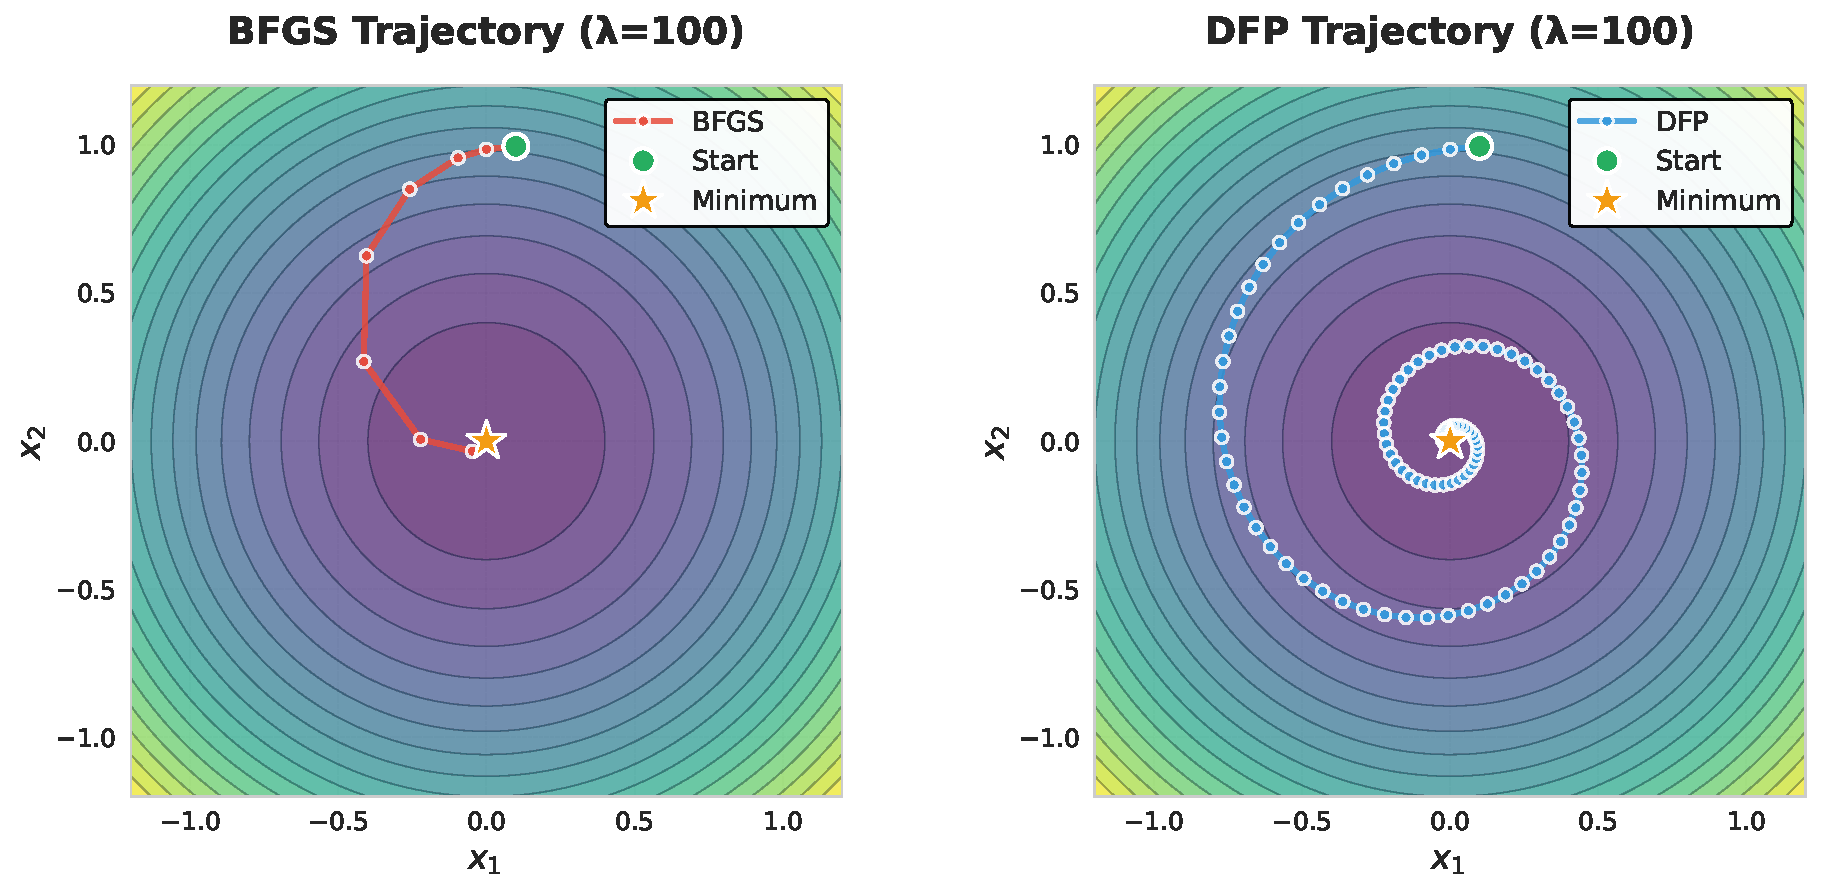
\includegraphics[width=\textwidth]{../imgs/quasi_newton/bfgs_vs_dfp_100.pdf}
    \caption{
        \ifEn
            Iterative trajectories for BFGS and DFP methods when $\lambda_1 = 100$. BFGS converges in 10 iterations while DFP requires 107 iterations, showing BFGS's superior efficiency for large eigenvalue errors.
        \else
            $\lambda_1 = 100$ におけるBFGSとDFPの反復軌跡。BFGSは10回で収束する一方、DFPは107回を要し、固有値誤差が大きい場合にBFGSが優位であることを示しています。
        \fi
    }
    \label{fig:bfgs_dfp_100}
\end{figure}

\begin{figure}[t]
    \centering
    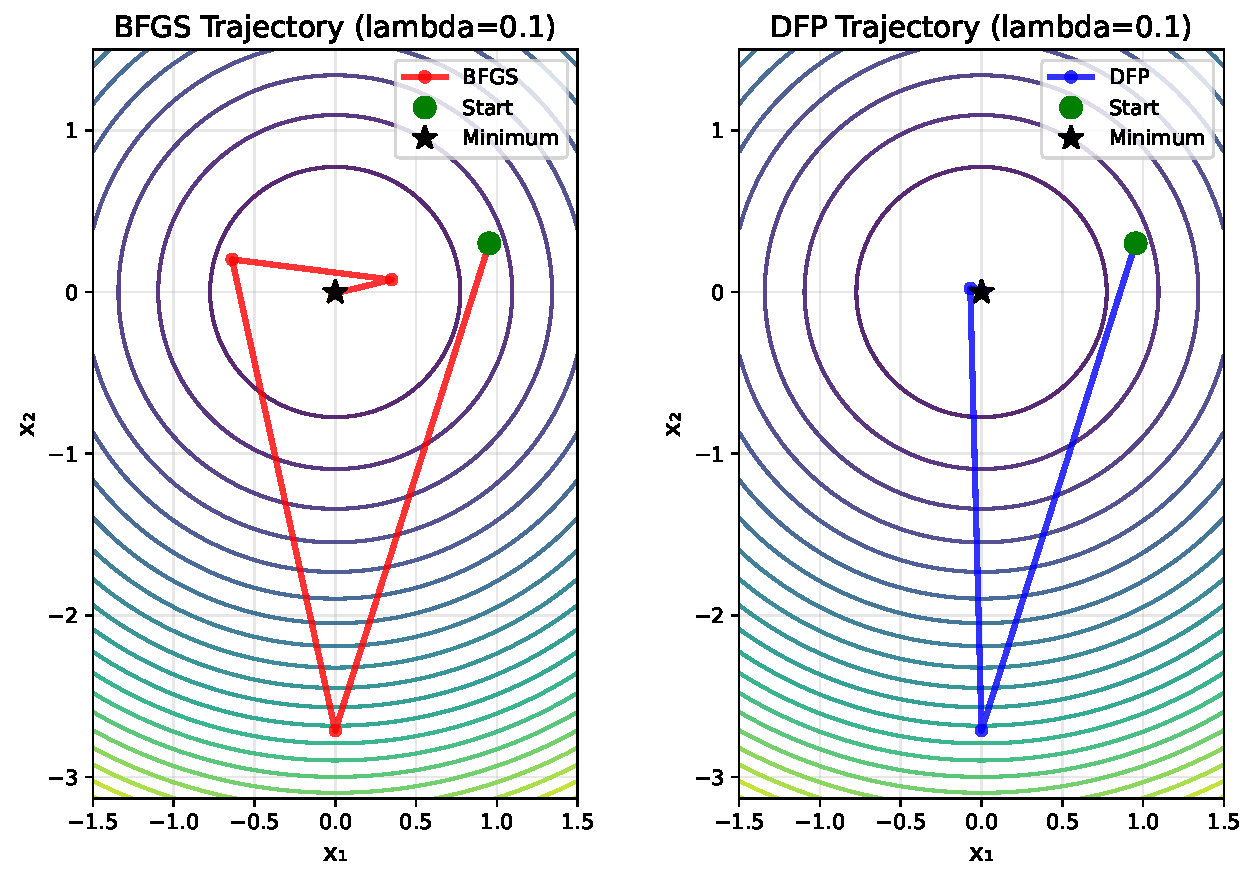
\includegraphics[width=\textwidth]{../imgs/quasi_newton/bfgs_vs_dfp_0.1.pdf}
    \caption{
        \ifEn
            Iterative trajectories for BFGS and DFP methods when $\lambda_1 = 0.1$. Both methods converge quickly, with DFP slightly faster than BFGS.
        \else
            $\lambda_1 = 0.1$ におけるBFGSとDFPの反復軌跡。どちらも素早く収束し、DFPがBFGSよりわずかに速くなっています。
        \fi
    }
    \label{fig:bfgs_dfp_0p1}
\end{figure}

\ifEn
    \subsubsection{Analysis and Discussion}
\else
    \subsubsection{解析と議論}
\fi

\ifEn
    The numerical results reveal a striking asymmetry between BFGS and DFP.
    When $\lambda_1 > 1$ (i.e., the initial Hessian approximation overestimates the true Hessian curvature), BFGS demonstrates significantly better efficiency.
    Conversely, when $\lambda_1 < 1$ (i.e., the initial Hessian approximation underestimates the true curvature), DFP performs slightly better than BFGS, though the difference is modest.
    This trend reversal is predicted by the theoretical symmetry between the two methods, but the magnitude of the difference is notable.
\else
    数値結果はBFGSとDFPの間に顕著な非対称性があることを示しています。
    $\lambda_1 > 1$ のとき、すなわち初期ヘッセ近似が真の曲率を過大評価する場合、BFGS は大幅に高い効率を示しました。
    一方で、 $\lambda_1 < 1$ のとき、すなわち初期ヘッセ近似が真の曲率を過小評価する場合には、DFPはBFGSよりわずかに良い性能を示しましたが、その差は非常に小さいものでした。
    この傾向の逆転は理論的な対称性から予測されるものですが、その差の大小は注目に値します。
\fi

\ifEn
    \paragraph{Asymmetry in Hessian Correction}
\else
    \paragraph{ヘッセ行列の補正における非対称性}
\fi

\ifEn
    The asymmetry of the performance arises from a fundamental difference in how these two methods correct erroneous eigenvalues.
    The core insight is that correcting erroneously large eigenvalues is more critical than correcting erroneously small ones.

    When a Hessian eigenvalue is overestimated, the algorithm takes steps that are too conservative, resulting in slow progress of the optimization.
    Correcting such errors requires the update formula to reduce these large eigenvalues toward one.
    The BFGS update is highly effective at this task, while the DFP update struggles.

    In contrast, when a Hessian eigenvalue is underestimated, the algorithm takes steps that are slightly too aggressive, but the error is self-correcting.
    Subsequent gradient computations provide information that helps refine the approximation.
    Thus, correcting underestimated eigenvalues is inherently easier and requires fewer iterations.

    This explains why the asymmetry in performance exists between BFGS and DFP.
\else
    両者の性能の非対称性は、誤った固有値を補正する仕方の根本的な違いに起因します。
    大事な考察として、過大な固有値の補正が過小な固有値の補正よりも重要であることが挙げられます。

    ヘッセ固有値が過大評価されると、アルゴリズムは過度に保守的なステップを取り、最適化の進みが遅くなります。
    この誤差を補正するには、更新則が大きな固有値を 1 へ縮小する必要があります。
    BFGS更新はこのようなタスクには強い効果を発揮しますが、DFP更新は苦手です。

    一方で、ヘッセ固有値が過小評価されると、アルゴリズムは大胆なステップを取りますが、その過小評価は自動で修正されやすいです。
    新しい点での勾配計算が近似の改善を促す為、このような過小評価の補正は本質的に容易で、必要な反復回数も少なくて済みます。

    このような差異が、BFGS更新とDFP更新の性能の非対称性を生み出していると考えることが出来ます。
\fi


\ifEn
    \subsection{Limited Memory BFGS (L-BFGS)}
\else
    \subsection{記憶制限BFGS (L-BFGS)}
\fi

\ifEn
    Next, we discuss the limited memory quasi-Newton methods, which are crucial for extending quasi-Newton methods to large-scale optimization problems.
    In standard quasi-Newton methods, the approximate Hessian $B_k$ or its inverse $H_k$ is stored and updated explicitly as a dense matrix, requiring $\mathcal{O}(n^2)$ memory for $n$ variables.
    In contrast, limited memory quasi-Newton methods maintain only a limited amount of information, i.e., the most recent $m$ curvature pairs $\{(s_i,y_i)\}$ and perform computations related to the approximate Hessian using just this information.
    This reduces the space complexity to $\mathcal{O}(nm)$, which is a dramatic improvement when $m$ is a small constant (typically $m\le 10$).
    The L-BFGS method~\citep{liuLimitedMemoryBFGS1989a}, which is a limited memory version of the BFGS update, is particularly representative.
    We focus on this BFGS update case and show how the quasi-Newton direction $d_k = -H_k g_k$ can be computed efficiently in terms of both space and time complexity using only the limited information.
\else
    以下では、準ニュートン法を大規模最適化問題へ拡張する際に重要となる、記憶制限準ニュートン法について説明します。
    通常の準ニュートン法では、近似ヘッセ行列 $B_k$ またはその逆行列 $H_k$ を密行列として陽に保存・更新するため、$n$ 変数に対して $\mathcal{O}(n^2)$ のメモリを要します。
    一方で、記憶制限準ニュートン法では、最新の $m$ 組のベクトルペア $\{(s_i,y_i)\}$ という限られた情報のみを保持して、その情報だけから近似ヘッセ行列に関する計算を行います。
    この工夫により空間計算量は $\mathcal{O}(nm)$ に減少し、$m$ が小さな定数(通常は $m\le 10$) のとき大幅な改善となります。
    特に、BFGS更新の記憶制限版であるL-BFGS法~\citep{liuLimitedMemoryBFGS1989a}は、特にその代表的な手法です。
    このBFGS更新の場合に注目し、限られた情報だけを用いて準ニュートン方向 $d_k = -H_k g_k$ を空間計算量・時間計算量の両面で効率的に計算する方法を示します。
\fi

\ifEn
    Throughout this subsection, we work with a finite sequence of matrices
\else
    本小節では次の有限長の行列の列を扱います。
\fi
\begin{equation*}
    H_0, H_1, \dots, H_m.
\end{equation*}
\ifEn
    Here, $H_\ell$ denotes the inverse Hessian approximation obtained after $\ell$ BFGS updates applied to a given initial matrix $H_0$.
\else
    ここで $H_\ell$ は初期行列 $H_0$ に対して $\ell$ 回のBFGS更新を適用して得られる逆ヘッセ近似を表します。
\fi

\ifEn
    \subsubsection{Compact Representation of the Inverse Hessian}
\else
    \subsubsection{逆行列のコンパクト表現}
\fi

\ifEn
    Let $\{(s_i,y_i)\}_{i=0}^{m-1}$ be the stored correction pairs, and define
\else
    保存されたベクトルペア $\{(s_i,y_i)\}_{i=0}^{m-1}$ を用いて、次を定義します。
\fi
\begin{equation*}
    \rho_i = \frac{1}{y_i^\top s_i}, \qquad
    V_i = I - \rho_i y_i s_i^\top.
\end{equation*}
\ifEn
    Then, for $i = 0,\dots, m-1$, the inverse BFGS update can be expressed as
\else
    このとき、 $i = 0,\dots, m-1$ に対して、BFGS更新の逆行列は次のように表されます。
\fi
\begin{equation*}
    H_{i+1} = V_i^\top H_i V_i + \rho_i s_i s_i^\top.
\end{equation*}
\ifEn
    By recursively expanding this relation, we obtain the compact representation
\else
    この関係を再帰的に展開すると次のコンパクト表現が得られます。
\fi
\begin{equation*}
    H_m
    =
    V_{m-1}^\top \cdots V_0^\top H_0 V_0 \cdots V_{m-1}
    +
    \sum_{j=0}^{m-1}
    (V_{m-1}^\top \cdots V_{j+1}^\top)
    \rho_j s_j s_j^\top
    (V_{j+1} \cdots V_{m-1}).
\end{equation*}
\ifEn
    Here, $H_0$ denotes the chosen initial inverse Hessian approximation, typically a scaled identity matrix.
\else
    ここで $H_0$ は選ばれた初期逆ヘッセ近似であり、通常はスケールされた単位行列です。
\fi

\ifEn
    \subsubsection{Two-Loop Recursion}
\else
    \subsubsection{二重ループ再帰}
\fi

\ifEn
    In quasi-Newton methods, it is crucial for the algorithm to efficiently compute $r = H_m q$ for the inverse matrix $H_m$ and a given vector $q \in \mathbb{R}^n$.
    This operation can be carried out using two short loops of length $m$, known as the L-BFGS two-loop recursion~\citep[Algorithm 7.4]{nocedal1999numerical}.
    This algorithm requires $\mathcal{O}(nm)$ time and space complexity.
\else
    準ニュートン法では、逆行列 $H_m$ と与えられたベクトル $q \in \mathbb{R}^n$ に対して $r = H_m q$ が効率的に計算できることが、アルゴリズムにおいて重要です。
    この計算は長さ $m$ の短いループを二回回すだけで実行でき、L-BFGS のtwo-loop recursionと呼ばれるアルゴリズムとして知られています~\citep[Algorithm 7.4]{nocedal1999numerical}。
    このアルゴリズムは $\mathcal{O}(nm)$ の時間・空間計算量を要します。
\fi

\subfile{999_two_loop_recursion.tex}

\ifEn
    In the following, we verify that the output of this two-loop recursion algorithm indeed computes $r = H_m q$.
\else
    この二重ループ再帰の出力が確かに $r = H_m q$ を計算していることを、以下では確認します。
\fi
\begin{proposition}
    \ifEn
        The output of the two-loop recursion algorithm satisfies $r = H_m q$.
    \else
        二重ループ再帰アルゴリズムの出力は $r = H_m q$ を満たす。
    \fi
\end{proposition}
\begin{proof}
    \ifEn
        In the first loop of the algorithm ($i = m-1, m-2, \dots, 0$), from the input vector $q^{(m)} \coloneqq q$, the algorithm computes
    \else
        アルゴリズムの1つ目のループ ($i = m-1, m-2, \dots, 0$) では、入力ベクトル $q^{(m)} \coloneqq q$ から次を計算する。
    \fi
    \begin{equation*}
        \alpha_i \coloneqq \rho_i s_i^\top q^{(i+1)}, \qquad
        q^{(i)} \coloneqq q^{(i+1)} - \alpha_i y_i.
    \end{equation*}
    \ifEn
        Substituting the definition of $\alpha_i$ and using the definition of $V_i$ in the compact representation, we find
    \else
        $\alpha_i$ の定義を代入し、コンパクト表現における $V_i$ の定義を用いると
    \fi
    \begin{equation*}
        q^{(i)} = q^{(i+1)} - \rho_i \left(s_i^\top q^{(i+1)}\right) y_i = \left(I - \rho_i y_i s_i^\top\right) q^{(i+1)} = V_i q^{(i+1)}.
    \end{equation*}
    \ifEn
        Thus, for all $i = 0, 1, \dots, m-1$, we have
    \else
        よってすべての $i = 0, 1, \dots, m-1$ に対して、次が得られます。
    \fi
    \begin{equation*}
        q^{(i)} = V_i V_{i+1} \cdots V_{m-1} q.
    \end{equation*}
    \ifEn
        Then, the algorithm applies $H_0$:
    \else
        次にアルゴリズムは $H_0$ を適用します。
    \fi
    \begin{equation*}
        r^{(0)} = H_0 q^{(0)} = H_0 V_0 V_1 \cdots V_{m-1} q.
    \end{equation*}
    \ifEn
        Next, for $i = 0, 1, \dots, m-1$, the second loop computes
    \else
        続いて、$i = 0, 1, \dots, m-1$ に対して、二つ目のループは次を計算します。
    \fi
    \begin{equation*}
        \beta_i     = \rho_i y_i^\top r^{(i)}, \qquad
        r^{(i+1)}   = r^{(i)} + s_i \left(\alpha_i - \beta_i\right).
    \end{equation*}
    \ifEn
        Substituting the definitions of $\alpha_i$, $\beta_i$, and $q^{(i+1)}$, we have
    \else
        $\alpha_i$, $\beta_i$, $q^{(i+1)}$ の定義を代入すると
    \fi
    \begin{align*}
        r^{(i+1)}
         & =
        r^{(i)} + \rho_i s_i s_i^\top \left(V_{i+1} V_{i+2} \cdots V_{m-1}\right) q - \rho_i s_i y_i^\top r^{(i)}            \\
         & = \left(I- \rho_i y_i s_i^\top\right) r^{(i)} + \rho_i s_i s_i^\top \left(V_{i+1} V_{i+2} \cdots V_{m-1}\right) q \\
         & =
        V_i^\top r^{(i)}
        +
        \rho_i s_i s_i^\top
        \left(V_{i+1} V_{i+2} \cdots V_{m-1}\right) q.
    \end{align*}
    \ifEn
        By recursively expanding this relation from the initial value $r^{(0)} = H_0 q^{(0)}$, we obtain
    \else
        初期値 $r^{(0)} = H_0 q^{(0)}$ からこの関係を再帰的に展開すると
    \fi
    \begin{equation*}
        r^{(m)}
        =
        V_{m-1}^\top \cdots V_0^\top H_0 V_0 \cdots V_{m-1} q
        +
        \sum_{j=0}^{m-1}
        (V_{m-1}^\top \cdots V_{j+1}^\top)
        \rho_j s_j s_j^\top
        (V_{j+1} \cdots V_{m-1}) q.
    \end{equation*}
    \ifEn
        This matches the compact representation of $H_m$ applied to $q$, and thus we have shown that the output of the algorithm satisfies $r = H_m q$, completing the proof.
    \else
        これは、$H_m$ のコンパクト表現を $q$ に適用した式と一致します。よって、アルゴリズムの出力が $r = H_m q$ を満たすことが示され、証明が完了します。
    \fi
    \myQED
\end{proof}

\ifEn
    Thus, the two-loop recursion exactly evaluates the action of the matrix $H_m$ on a vector without explicitly constructing the matrix $H_m$.
\else
    従って、このtwo-loop recursionによって、行列 $H_m$ を陽に構成せずに、ベクトルに対する作用を正確に評価できることがわかります。
\fi

\ifEn
    \subsubsection{Initial Step Size}
\else
    \subsubsection{初期スケーリング}
\fi

\ifEn
    A crucial component of the L-BFGS method is the choice of the initial matrix $H_0$.
    A widely used option is a scaled identity:
\else
    L-BFGS 法の重要な要素は初期行列 $H_0$ の選択です。
    広く使われるのは、単位行列にスケーリングを施したものです。
\fi
\begin{equation*}
    H_0 = \gamma I.
\end{equation*}
\ifEn
    Here, the scaling parameter $\gamma$ is often chosen as
\else
    ここでスケーリング係数 $\gamma$ は、例えば次のように選ばれます。
\fi
\begin{equation*}
    \gamma = \frac{s_{m-1}^\top y_{m-1}}{y_{m-1}^\top y_{m-1}}.
\end{equation*}
\ifEn
    This choice is motivated by the following discussion~\citep{liuLimitedMemoryBFGS1989a,shannoMatrixConditioningNonlinear1978}.
    Assume that the objective function $f$ is twice continuously differentiable and consider the mean Hessian along the most recent step:
\else
    この選択は次の議論によって正当化できます~\citep{liuLimitedMemoryBFGS1989a,shannoMatrixConditioningNonlinear1978}。
    目的関数 $f$ が二回連続微分可能であると仮定し、最新のステップに沿った平均ヘッセ行列を考えます。
\fi
\begin{equation*}
    \bar{G} = \int_0^1 \nabla^2 f(x + \tau s_{m-1}) \mathrm{d}\tau.
\end{equation*}
\ifEn
    Recall that $s_{m-1}$ denotes the most recent displacement of $x$, satisfying
\else
    ここで $s_{m-1}$ は最新の $x$ の変位を表しており、次を満たします。
\fi
\begin{equation*}
    y_{m-1}
    =
    \nabla f(x+s_{m-1}) - \nabla f(x)
    =
    \bar{G} s_{m-1}.
\end{equation*}
\ifEn
    Using this relation, the scaling factor can be written as
\else
    この関係を用いるとスケーリング係数は次のように書けます。
\fi
\begin{equation*}
    \frac{s_{m-1}^\top y_{m-1}}{y_{m-1}^\top y_{m-1}}
    =
    \frac{(\bar{G}^{1/2} s_{m-1})^\top (\bar{G}^{1/2} s_{m-1})}
    {(\bar{G}^{1/2} s_{m-1})^\top \bar{G} (\bar{G}^{1/2} s_{m-1})}.
\end{equation*}
\ifEn
    This is a reciprocal of a Rayleigh quotient of the matrix $\bar{G}$ with respect to the vector $\bar{G}^{1/2} s_{m-1}$.
    Therefore, this scaling roughly approximates the average inverse curvature along those directions.
\else
    これは、ベクトル $\bar{G}^{1/2} s_{m-1}$ に関する行列 $\bar{G}$ のRayleigh商の逆数です。
    従って、このスケーリングはこれらの方向に沿った平均逆曲率を大まかに近似しています。
\fi

\ifEn
    Moreover, this choice of $\gamma$ coincides with the short step size of the Barzilai--Borwein method~\citep{barzilaiTwoPointStepSize1988}, highlighting a close connection between L-BFGS initialization and classical step-length selection strategies.
\else
    さらにこの $\gamma$ の選択は Barzilai--Borwein 法の短ステップサイズ~\citep{barzilaiTwoPointStepSize1988} と一致しており、L-BFGS の初期化と古典的なステップ長選択戦略の密接な関係を示しています。
\fi

\ifSubfilesClassLoaded{
    \bibliographystyle{plainnat}
    \bibliography{../L-BFGS.bib}
}{}

\end{document}